\documentclass[a4paper]{report} % set paper size

\usepackage[utf8]{inputenc}
\usepackage {url}
\usepackage[top=2.0cm, bottom=2.0cm, left=2.54cm, right=2.54cm]{geometry} % set margin
\usepackage{amsfonts} % for set names
\usepackage{amsmath} % for equation system
\usepackage{amsthm} % for theorem block
\usepackage{fixltx2e} % for subscript
\usepackage{fancyhdr} % for footer/headline modification
\usepackage{xcolor}
\usepackage{graphicx} % for image insertion
\usepackage[ruled,vlined]{algorithm2e} % for algorithm integration

\pagestyle{fancyplain} % for footing modification on all pages
\fancyhf{}
%\renewcommand{\headrulewidth}{0pt} % remove decorative lign
\fancyhead[L]{Pauline Maury Laribiere, Alexandre Devienne}
\fancyhead[R]{MT/EL-BA2 EPFL 2015}
\fancyhead[C]{\textbf{Spring programming project : Microcosmos}}

\fancyfoot[R]{\thepage\ of \pageref{lastpage}}

\begin{document}

% =====================================================================
\section{Program's architecture}
\begin{figure}
\begin{center}
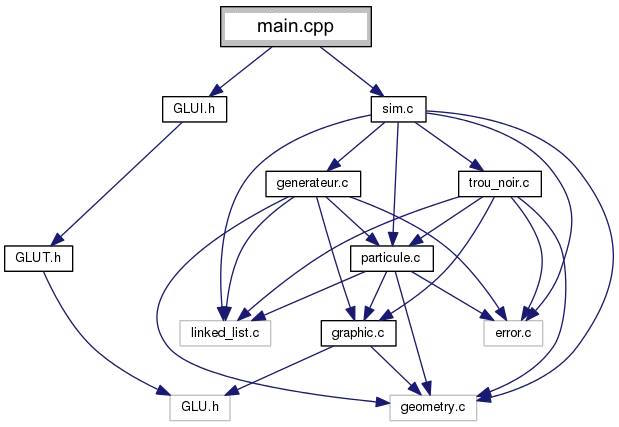
\includegraphics[scale=0.6]{architecture.jpg}
\end{center}
\caption{Final architecture}
\end{figure}

Compared to the architecture suggested, we added two low level modules:
\begin{description}
\item[geometry]
Low level representation of points and vectors and functions to manipulate them (ex: distance between points, norm of a vector)

This module in included in the modules : \emph{main}, \emph{sim}, \emph{generateur}, \emph{particule}, \emph{trou\_noir}, \emph{graphic}.
\item[linked\_list]
Abstract double linked list data structure.
Some basic dictionary are implemented such as : first, next, add, delete, search
More complex operations exist such as : sorting and calling a function with 2 elements as argument , for every possible 2-combinations of elements
(to work out the forces between every particles for example)

This module in included in the modules : \emph{sim}, \emph{generateur}, \emph{particule}, \emph{trou\_noir}.
\end{description}

Working with these modules eases our work by reducing the amount of redundant.
It also eased the testing part, as we could validate the correctness of these modules before using them in the project.
Indeed, we created a special test environment unrelated to the project to test them.

Compared to the architecture suggested, we also added 2 dependency:
\begin{description}
\item[trou\_noir -> particule]
This allows \emph{trou\_noir} to call \text{void part\_applyForceField( void (*forceFieldAt) (POINT p) )}
to apply the force generated by all black holes to all particles .
Plus, to destroy particles too close to a black hole, it can call \text{int part\_closestPartOn( POINT p )}
to retrieve a particle's ID to then destroy it with : \text{bool part\_delete( int partID )}

\item[generateur -> particule]
This allows \emph{generateur} to delegate the validity of a generator's argument to \emph{particule}
and to create particle by a simple call of \text{part\_create}j
\end{description}

% =====================================================================
\section{Data structures}



% =====================================================================
\section{Function called by \text{main.cpp} from \text{sim.c}
Here are the different functions of sim.c called in main.cpp :

First, there are functions provided for the file management : sim_openFile that manages the different 
mode supported by the simulation and sim_save that saves  the current state of the simulation in a file.

Then, some functions purpose's is to get the information :  sim_nbEntities updates the number of each entity and 
sim_extremPoints returns the outermost points at the beginning of the simulation to calculate the frame of the window to open.

Other functions handles the advancement of the simulation : sim_display that calls the different entities to 
display them and sim_next_step that handles calculation for the next step of the simulation.

Thare are also functions dedicated to the input : sim_select enables the user of the program to select 
an entity, sim_deleteSelection to delete it and sim_unselect to unselect a selected entity.

Finally, sim_clean object is to free memory from all modules accross the simulation.

\label{lastpage}
\end{document}
